\section{手工例题}
\subsection{有效集方法}
\begin{figure}[H]
    \centering
    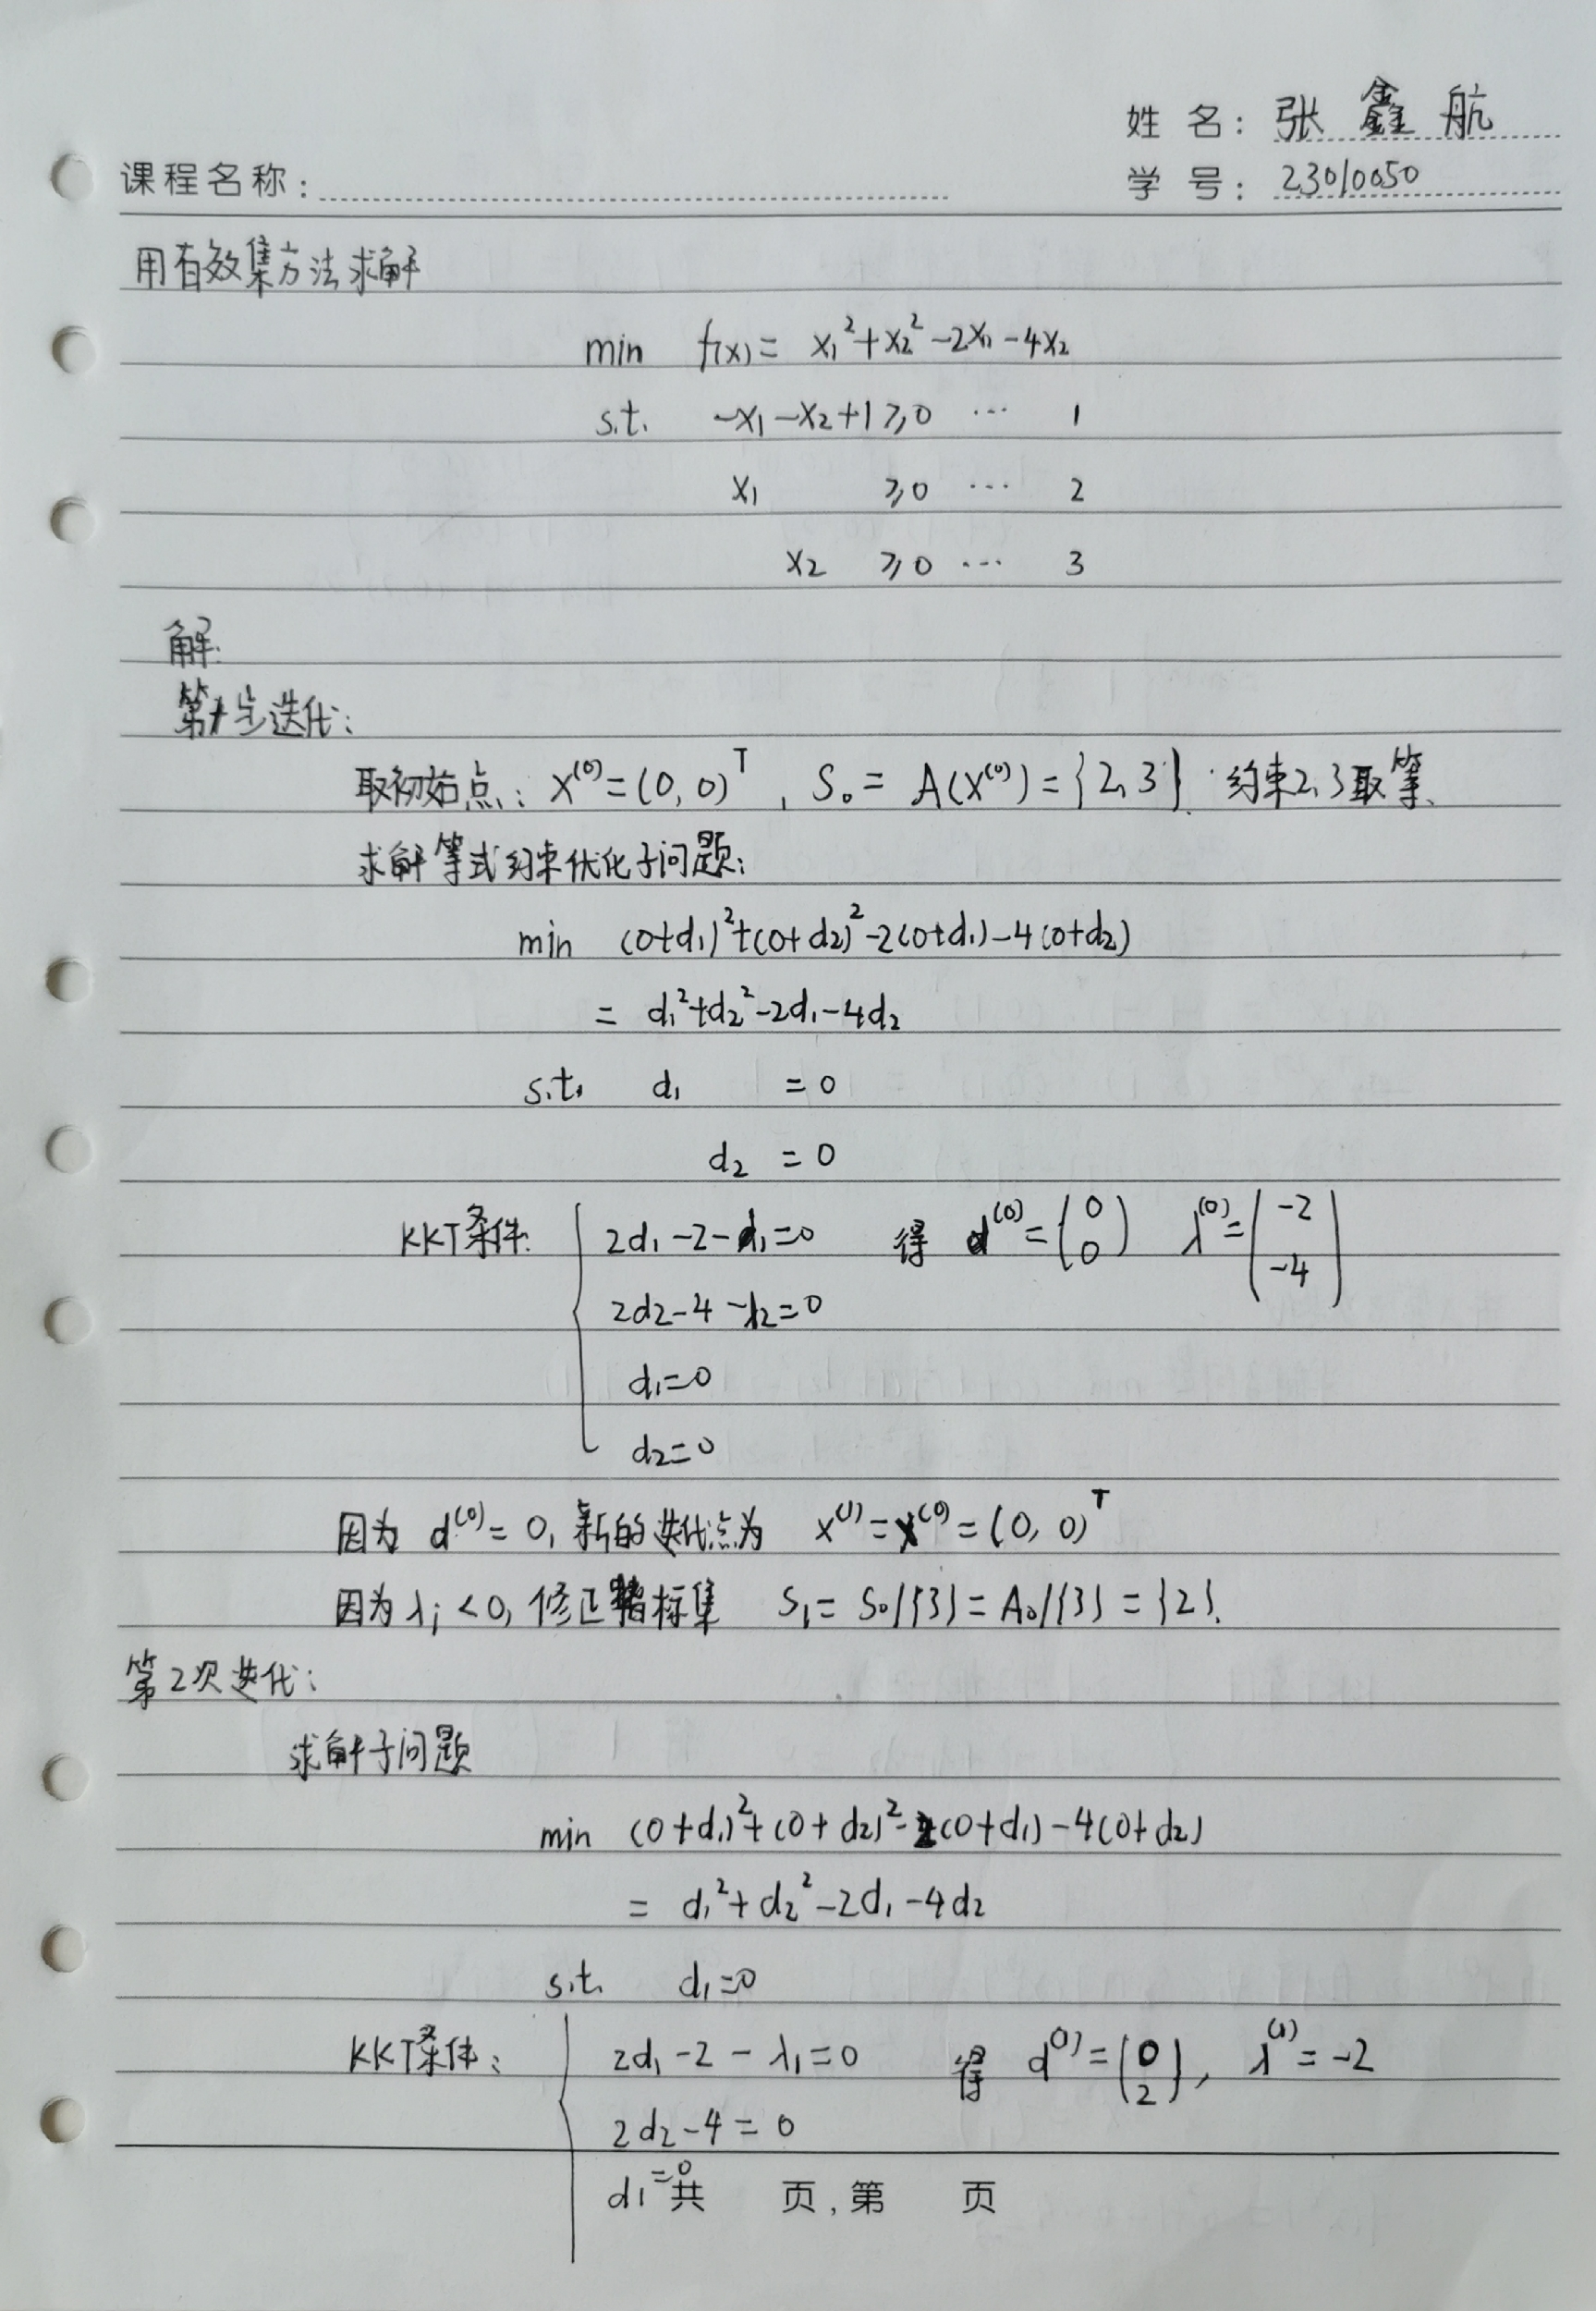
\includegraphics[width = \textwidth]{data/手写-有效集方法-1.jpg}
\end{figure}
\begin{figure}[H]
    \centering
    \includegraphics[width = \textwidth]{data/手写-有效集方法-2.jpg}
\end{figure}
\begin{example}
    求解二次规划问题\Stars{5}{}
    \begin{equation}\label{eq:hand-calculation}
        \begin{array}{rl}
            \operatorname*{min} & Q(\boldsymbol{x})=x_{1}^{2}+x_{2}^{2}-2x_{1}-4x_{2}\\
            \mathrm{s.t.}&-x_{1}-x_{2}+1\geqslant0\\
            &x_{1},x_{2}\geqslant 0
        \end{array}
    \end{equation}
    \begin{solution}
        \colorbox{cyan!50}{$k = 0$:}

        取初始点
        \[
            \boldsymbol{x}^{(0)}=\begin{pmatrix}0\\0\end{pmatrix},\, S_0=\mathcal{A}(\boldsymbol{x}^{(0)})=\{2,3\}
        \]
        求解等式约束优化子问题
        \[
            \begin{array}{rl}
                \min & d_{1}^{2}+d_{2}^{2}-2d_{1}-4d_{2}\\
                \mathrm{s.t.} & d_{1}=0\\
                & d_{2}=0
            \end{array}
        \]
        KKT条件
        \[
            \left\{
                \begin{array}{l}
                    2d_1-2-\lambda_1 = 0\\
                    2d_2-4-\lambda_2 = 0\\
                    d_1 = 0\\
                    d_2 = 0
                \end{array}
            \right.
        \]
        得最优解和相应的Lagrange乘子
        \[
            \boldsymbol{d}^{(0)}=\begin{pmatrix}0\\0\end{pmatrix},\,
            \boldsymbol{\lambda}^{(0)}=\begin{pmatrix}-2\\-4\end{pmatrix}
        \]
        因为$\boldsymbol{d}^{(0)} = \boldsymbol{0}$,新的迭代点为
        \[
            \boldsymbol{x}^{(1)}= \boldsymbol{x}^{(0)} = \begin{pmatrix}0\\0\end{pmatrix}
        \]
        因为$\lambda_{i} <0$,修正指标集
        \[
            S_1=S_0/\{3\}=\mathcal{A}_0/\{3\}=\{2\}
        \]

        \colorbox{cyan!50}{$k = 1$:}

        求解子问题
        \[
            \begin{array}{rl}
                \operatorname*{min}&d_{1}^{2}+d_{2}^{2}-2d_{1}-4d_{2}\\
                \mathrm{s.t.}&d_{1}=0
            \end{array}
        \]
        KKT条件
        \[
            \left\{
                \begin{array}{l}
                    2d_1-2-\lambda_1 = 0\\
                    2d_2-4 = 0\\
                    d_1 = 0\\
                \end{array}
            \right.
        \]
        得最优解
        \[
            \boldsymbol{d}^{(1)}=\begin{pmatrix}0\\2\end{pmatrix},\,
            \boldsymbol{\lambda}^{(1)}=\begin{pmatrix}-2\end{pmatrix}
        \]  
        因为$\boldsymbol{d}^{(1)}\neq \boldsymbol{0}$,转第三步,计算步长$\alpha$,其中$i\in\mathcal{I}/S_{1} = \left\{ 1,2,3 \right\}/\left\{ 2 \right\} = \left\{ 1,3 \right\}$
        \newline
        因为
        \[
            \begin{array}{l}
                \boldsymbol{a}_{1}^{\mathrm{T}}\boldsymbol{d}^{(1)} =
                \begin{pmatrix}
                    -1 & -1
                \end{pmatrix}\cdot
                \begin{pmatrix}
                    0 \\ 2
                \end{pmatrix} = -2 \\
                \boldsymbol{a}_{2}^{\mathrm{T}}\boldsymbol{d}^{(1)}  =
                \begin{pmatrix}
                    0 & 1
                \end{pmatrix}\cdot
                \begin{pmatrix}
                    0 \\ 2
                \end{pmatrix} = 2>0
            \end{array}
        \]
        \[
            \begin{aligned}
                \alpha_{1}& =\min\left\{1,\frac{b_{i}-\boldsymbol{a}_{i}^{\mathrm{T}}\boldsymbol{x}^{(1)}}{\boldsymbol{a}_{i}^{\mathrm{T}}\boldsymbol{d}^{(1)}}\mid i=1,3,\boldsymbol{a}_{i}^{\mathrm{T}}\boldsymbol{d}^{(1)}<0\right\}  \\
                &=\min\left\{1,\dfrac{-1-\begin{pmatrix}
                    -1 & -1
                \end{pmatrix}\cdot
                \begin{pmatrix}
                    0 \\ 0
                \end{pmatrix}}{-2}\right\} = \dfrac{1}{2}
            \end{aligned}
        \]
        从$\mathcal{I}/S_{1} = \left\{ 1,3 \right\}$中取
        \[
            \begin{array}{l}
                \boldsymbol{a}_{1}^{\mathrm{T}}\boldsymbol{x}^{(2)} = \begin{pmatrix}
                    -1 & -1
                \end{pmatrix}\cdot
                \begin{pmatrix}
                    0 \\ 1
                \end{pmatrix} = -1 =
                \boldsymbol{b}_1 \\
                \boldsymbol{a}_{3}^{\mathrm{T}}\boldsymbol{x}^{(2)} = \begin{pmatrix}
                    0 & 1
                \end{pmatrix}\cdot
                \begin{pmatrix}
                    0 \\ 1
                \end{pmatrix} = -1 \neq
                \boldsymbol{b}_3 = 0
            \end{array}
        \]
        不等式积极约束$i = 1$
        令
        \[
            \boldsymbol{x}^{(2)}=\boldsymbol{x}^{(1)}+\alpha_1\boldsymbol{d}^{(1)}=\begin{pmatrix}0\\1\end{pmatrix},\,S_2 = S_1\cup \{1\} = \{1,2\}
        \]

        \colorbox{cyan!50}{$k = 3$:}

        求解子问题
        \[
            \begin{array}{rl}
                \operatorname*{min}&d_{1}^{2}+d_{2}^{2}-2d_{1}-2d_{2}\\
                \mathrm{s.t.}&-d_{1}-d_2=0\\
                &d_1 = 0
            \end{array}
        \]
        KKT条件
        \[
            \left\{
                \begin{array}{l}
                    2d_1-2+\lambda_1 = 0\\
                    2d_2-2+\lambda_1-\lambda_2 = 0\\
                    d_1+d_2 = 0\\
                    d_1 = 0
                \end{array}
            \right.
        \]
        得最优解
        \[
            \boldsymbol{d}^{(2)}=\begin{pmatrix}0\\0\end{pmatrix},\,\boldsymbol{\lambda}^{(2)}=\begin{pmatrix}2\\0\end{pmatrix}
        \] 
        由$\boldsymbol{d}^{(2)}=0$,且对于$\forall i\in S_{k}\cap \mathcal{I}(\boldsymbol{x}^{(2)}) = \left\{ 1,2 \right\},\lambda_{i}^{(2)}\geqslant 0$算法停止。原问题最优解和最优Lagrange乘子分别为:
        \[
            \boldsymbol{x}^*=\boldsymbol{x}^{(2)}=\begin{pmatrix}0\\1\end{pmatrix},\quad 
            \boldsymbol{\lambda}^* = \begin{pmatrix}
                2\\0\\0
            \end{pmatrix}
        \]
        \[
            f(\boldsymbol{x}^{*}) = -3
        \]
    \end{solution}
\end{example}
\subsection{共轭梯度法}
\begin{figure}[H]
    \centering
    \includegraphics[width = \textwidth]{data/手写-共轭梯度法.jpg}
\end{figure}
\begin{example}
    利用共轭梯度法求$\boldsymbol{Ax} = \boldsymbol{b}$或者说,利用共轭梯度法求$\min x_1^2+\dfrac{1}{2}x_2^2+\dfrac{1}{2}x_3^2$\quad\Stars{5}

    其中,
    \[
        \boldsymbol{A} = \begin{bmatrix}
            2 & 0 & 0\\
            0 & 1 & 0 \\
            0 & 0 & 1
        \end{bmatrix},\quad
        \boldsymbol{b} = \begin{pmatrix}
            0\\0\\0
        \end{pmatrix}
    \]    
    \begin{solution}
        取初始点$\boldsymbol{x}_0 = (1,1,1)^{\mathrm{T}} $,迭代过程:
        \[
            \frac{\partial f}{\partial x_1} = 2x_1,\,\frac{\partial f}{\partial x_2} = x_2,\,\frac{\partial f}{\partial x_3} = 2x_3,
        \]
        \begin{enumerate}
            \item $\boldsymbol{x}_0 = (1,1,1)^{\mathrm{T}} $,$\boldsymbol{g}_0 = (2,1,1)^{\mathrm{T}}$,$\beta_{-1} = 0$,$\boldsymbol{d}_{0} = -\boldsymbol{g}_0 = (-2,-1,-1)^{\mathrm{T}}$.
            \[
                \begin{array}{ll}
                     f(\boldsymbol{x}_0+\alpha \boldsymbol{d}_0)&=f( (1-2\alpha),\frac{1}{2}(1-\alpha),\frac{1}{2}(1-\alpha) )\\
                    & = (1-2\alpha)^2+\frac{1}{2}(1-\alpha)^2+\frac{1}{2}(1-\alpha)^2\\
                    &=(4+\frac{1}{2}+\frac{1}{2})\alpha^2+(-4-1-1)\alpha+c
                \end{array}
            \]
            \[
                \alpha_0 = \arg\min f(\boldsymbol{x}_0+\alpha_0\boldsymbol{d}_0) = -\frac{-4-1-1}{2(4+\frac{1}{2}+\frac{1}{2})} = \frac{3}{5}
            \]
            \item $\boldsymbol{x}_1 = \boldsymbol{x}_0+\alpha_0\boldsymbol{d}_0=\frac{1}{5}(-1,2,2)^{\mathrm{T}} $,$\boldsymbol{g}_1 = \frac{2}{5}(-1,1,1)^{\mathrm{T}}$,$\beta_{0} = \frac{\boldsymbol{g}_1^{\mathrm{T}}\boldsymbol{g}_1}{\boldsymbol{g}_0^{\mathrm{T}}\boldsymbol{g}_0}= \frac{2}{25}$ 
            \[
                \boldsymbol{d}_{1} = -\boldsymbol{g}_1+\beta_{0}\boldsymbol{d}_0 = -\frac{6}{25}(1,-2,-2)^{\mathrm{T}}
            \]
            \[
                \begin{array}{ll}
                     f(\boldsymbol{x}_1+\alpha \boldsymbol{d}_1)&=f( (-\frac{1}{5}+\frac{6}{25}\alpha),\frac{1}{2}(\frac{2}{5}-\frac{12}{25}\alpha),\frac{1}{2}(\frac{2}{5}-\frac{12}{25}\alpha) )\\
                    &=\frac{1}{25^2}\left[ (36+72+72)\alpha^2+(-60-120-120)\alpha+c \right]
                \end{array}
            \]
            \[
                \alpha_1 = \arg\min f(\boldsymbol{x}_1+\alpha_1\boldsymbol{d}_1) = -\frac{-60-120-120}{2(36+72+72)} = \frac{5}{6}
            \]
            \item $\boldsymbol{x}_2 = \boldsymbol{x}_1 + \alpha_1\boldsymbol{d}_1 = \boldsymbol{0}$,$\|\boldsymbol{g}_2\| = 0$,终止。
        \end{enumerate}
        知道$\boldsymbol{x}^* = (0,0,0)^{\mathrm{T}},\,\min f(\boldsymbol{x}) = 0$,迭代过程如下:
        \begin{table}[htbp]
            \centering
            \begin{tabular}{c|c|c|c|c|c}
                \hline
                $k$ & $\boldsymbol{x}_k$ & $\boldsymbol{g}_k$ & $\beta_{k-1}$ & $\boldsymbol{d}_k$ & $\alpha_k$\\\hline
                $0$ & $ (1,1,1)^{\mathrm{T}} $ & $(2,1,1)^{\mathrm{T}}$ & $0$ & $ -(2,1,1)^{\mathrm{T}} $ & $\frac{3}{5}$\\\hline
                $1$ & $ \frac{1}{5}(-1,2,2)^{\mathrm{T}} $ & $\frac{1}{5}(-2,2,2)^{\mathrm{T}}$ & $\frac{2}{25}$ & $ -\frac{6}{25}(1,-2,-2)^{\mathrm{T}} $ & $\frac{5}{6}$\\\hline
                $2$ & $(0,0,0)^{\mathrm{T}}$ & $(0,0,0)^{\mathrm{T}}$ & \\\hline
            \end{tabular}
        \end{table}
    \end{solution}
\end{example}
\subsection{DFP}
\begin{figure}[htbp]
    \centering
    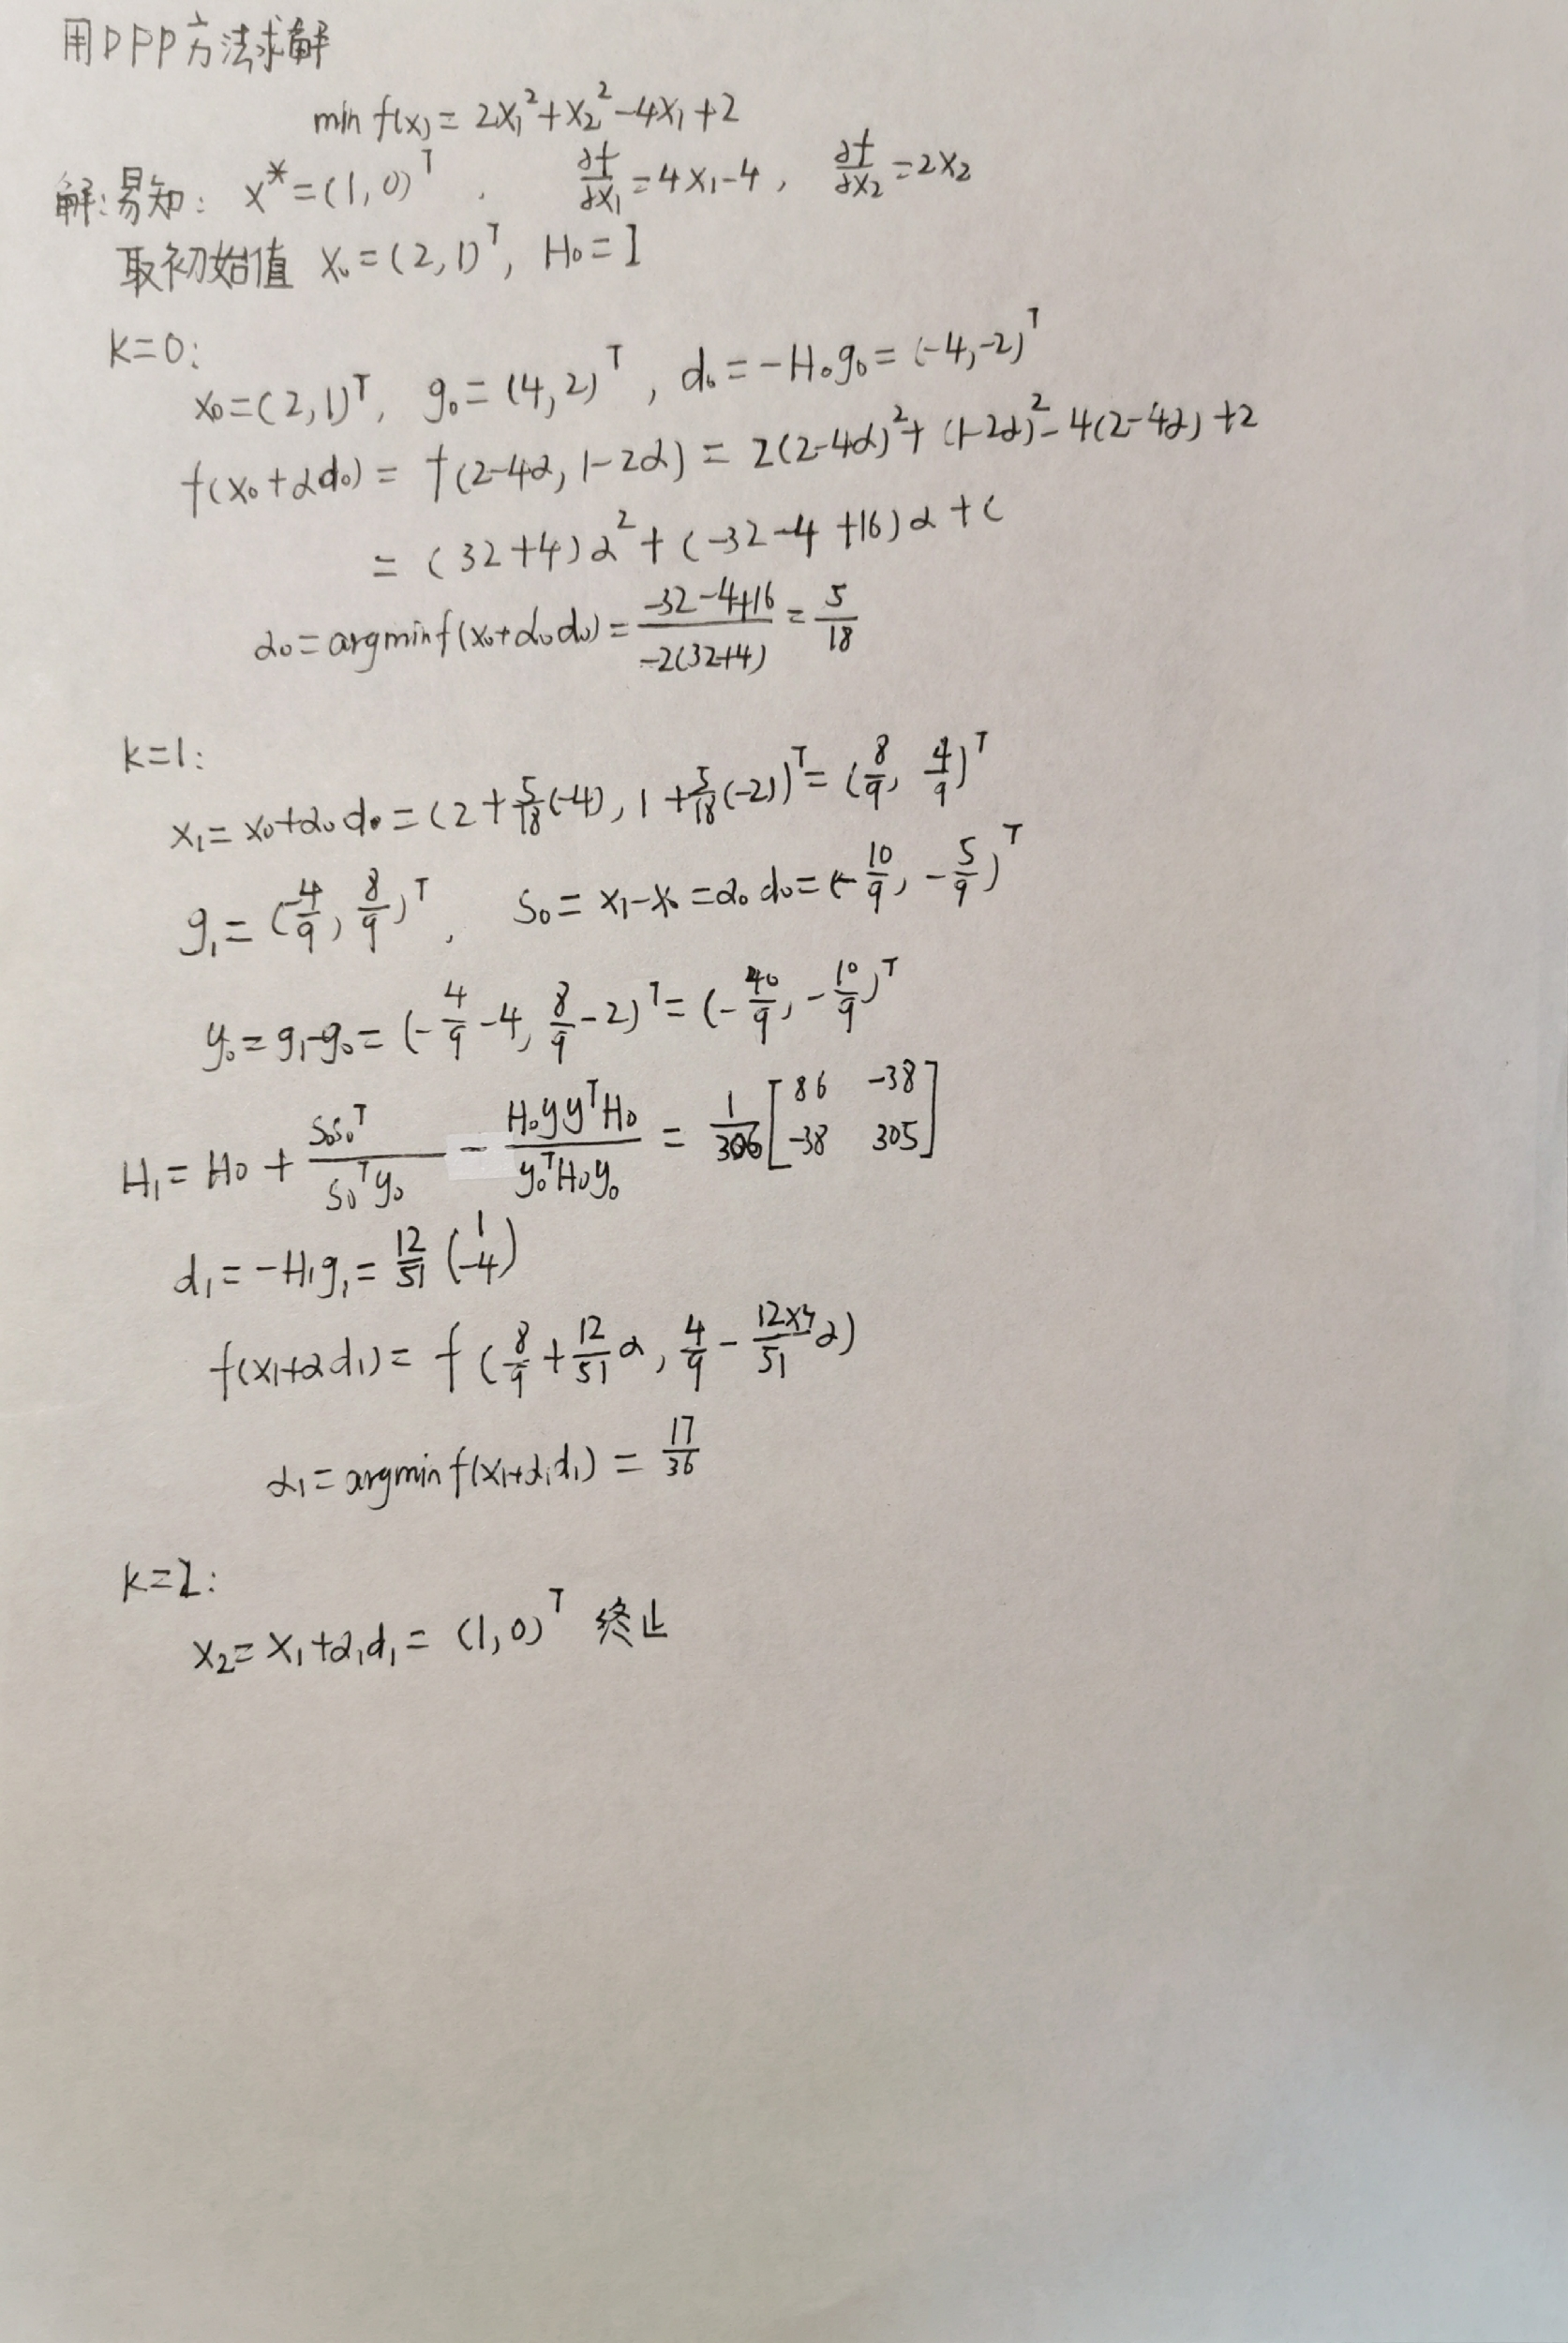
\includegraphics[width = \textwidth]{data/手写-DFP-1.jpg}
\end{figure}
\begin{figure}[htbp]
    \centering
    \includegraphics[width = \textwidth]{data/手写-DFP-2.jpg}
\end{figure}